\documentclass[10pt, UTF8]{article}
\usepackage[a4paper, scale = 0.8]{geometry}
\usepackage{ctex}

\usepackage{enumitem}
\usepackage{listings}
\usepackage{xcolor}
\usepackage{color}
\definecolor{GrayCodeBlock}{RGB}{241, 241, 241}
\definecolor{BlackText}{RGB}{0, 0, 0}
\definecolor{RedTypename}{RGB}{182, 86, 17}
\definecolor{GreenString}{RGB}{96, 172, 57}
\definecolor{PurpleKeyword}{RGB}{184, 84, 212}
\definecolor{GrayComment}{RGB}{170, 170, 170}
\definecolor{GoldDocumentation}{RGB}{180, 165, 45}
\lstset {
  columns = fullflexible, keepspaces = true, showstringspaces=false, breaklines = true, frame = single, framesep = 0pt, framerule = 0pt, framexleftmargin = 4pt, framexrightmargin = 4pt, framextopmargin = 5pt, framexbottommargin = 3pt, xleftmargin = 4pt, xrightmargin = 4pt,
  backgroundcolor = \color{GrayCodeBlock},
  basicstyle = \ttfamily\color{BlackText},
  keywordstyle = \color{PurpleKeyword},
  ndkeywordstyle = \color{RedTypename},
  stringstyle = \color{GreenString},
  commentstyle = \color{GrayComment}
}

\usepackage{graphicx}
\usepackage{amsmath}
\usepackage{multirow}

\usepackage[colorlinks, linkcolor = red, anchorcolor = blue, citecolor = green]{hyperref}

\renewcommand\thesection{\arabic{section}}

\title{数据挖掘第五次作业}
\author{李晨昊 2017011466}
\begin{document}
\maketitle
\tableofcontents

\section{决策树}

下表给出了两组人的数据,每组数据分别包含4个和5个样本。

\begin{table}[htbp]
\center
  \begin{tabular}{|c|c|c|c|c|}
    \hline
    组次                                                                 & id & 身材 & 发色 & 年龄 \\ \hline
    \multirow{4}{*}{\begin{tabular}[c]{@{}c@{}}第\\ 一\\ 组\end{tabular}} & 1  & 矮  & 金色 & 老人 \\ \cline{2-5} 
    & 2  & 高  & 红色 & 老人 \\ \cline{2-5} 
    & 3  & 高  & 金色 & 老人 \\ \cline{2-5} 
    & 4  & 矮  & 金色 & 成年 \\ \hline
    \multirow{5}{*}{\begin{tabular}[c]{@{}c@{}}第\\ 二\\ 组\end{tabular}} & 1  & 高  & 黑色 & 儿童 \\ \cline{2-5} 
    & 2  & 矮  & 黑色 & 老人 \\ \cline{2-5} 
    & 3  & 高  & 黑色 & 老人 \\ \cline{2-5} 
    & 4  & 高  & 黑色 & 成年 \\ \cline{2-5} 
    & 5  & 矮  & 金色 & 儿童 \\ \hline
  \end{tabular}
\end{table}

\begin{enumerate}
  \item 使用任意一种决策树方法建立该数据集的二分类器,使它能正确区分这两组人,写出建立过程。
  
  我选择使用ID3算法。表格中的id对分类无任何影响,而且因为两组间有相同的id,也不能用于区分元素,为了方便,我将第二组的编号1-5重新编号为5-9,这样id就可以用来区分元素。
  
  \begin{itemize}
    \item 剩余元素集合$\{1, 2, 3, 4, 5, 6, 7, 8, 9\}$,剩余属性集合$\{\text{身材}, \text{发色}, \text{年龄}\}$
    \begin{align*}
    Info(D) &= -(\frac{4}{9}\log_2{\frac{4}{9}} + \frac{5}{9}\log_2{\frac{5}{9}}) = 0.991 \\
    Info_{\text{身材}} &= -(\frac{4}{9}(\frac{2}{9}\log_2{\frac{2}{9}} + \frac{2}{9}\log_2{\frac{2}{9}}) + \frac{5}{9}(\frac{2}{9}\log_2{\frac{2}{9}} + \frac{3}{9}\log_2{\frac{3}{9}})) = 0.990  \\
    Info_{\text{发色}} &= -(\frac{4}{9}(\frac{3}{9}\log_2{\frac{3}{9}} + \frac{1}{9}\log_2{\frac{1}{9}}) + \frac{1}{9}(\frac{1}{9}\log_2{\frac{1}{9}} + \frac{0}{9}\log_2{\frac{0}{9}}) + \frac{4}{9}(\frac{0}{9}\log_2{\frac{0}{9}} + \frac{4}{9}\log_2{\frac{4}{9}})) = 0.662  \\
    Info_{\text{年龄}} &= -(\frac{5}{9}(\frac{3}{9}\log_2{\frac{3}{9}} + \frac{2}{9}\log_2{\frac{2}{9}}) + \frac{2}{9}(\frac{1}{9}\log_2{\frac{1}{9}} + \frac{1}{9}\log_2{\frac{1}{9}}) + \frac{2}{9}(\frac{0}{9}\log_2{\frac{0}{9}} + \frac{2}{9}\log_2{\frac{2}{9}})) = 0.825
    \end{align*}
    选择发色,分出$\{1, 3, 4, 9\}$和$\{2\}$和$\{5, 6, 7, 8\}$。
    \item 剩余元素集合$\{1, 3, 4, 9\}$,剩余属性集合$\{\text{身材}, \text{年龄}\}$
    \begin{align*}
    Info(D) &= -(\frac{3}{4}\log_2{\frac{3}{4}} + \frac{1}{4}\log_2{\frac{1}{4}}) = 0.811 \\
    Info_{\text{身材}} &= -(\frac{3}{4}(\frac{2}{4}\log_2{\frac{2}{4}} + \frac{1}{4}\log_2{\frac{1}{4}}) + \frac{1}{4}(\frac{1}{4}\log_2{\frac{1}{4}} + \frac{0}{4}\log_2{\frac{0}{4}})) = 0.875  \\
    Info_{\text{年龄}} &= -(\frac{2}{4}(\frac{2}{4}\log_2{\frac{2}{4}} + \frac{0}{4}\log_2{\frac{0}{4}}) + \frac{1}{4}(\frac{1}{4}\log_2{\frac{1}{4}} + \frac{0}{4}\log_2{\frac{0}{4}}) + \frac{1}{4}(\frac{0}{4}\log_2{\frac{0}{4}} + \frac{1}{4}\log_2{\frac{1}{4}})) = 0.500
    \end{align*}
    选择年龄,分出$\{1, 3\}$和$\{4\}$和$\{9\}$。
    \item 剩余元素集合$\{1, 3\}$,剩余属性集合$\{\text{身材}\}$
    。由于元素种类唯一,不再分类。
    \item 剩余元素集合$\{4\}$,剩余属性集合$\{\text{身材}\}$
    。由于元素种类唯一,不再分类。
    \item 剩余元素集合$\{9\}$,剩余属性集合$\{\text{身材}\}$
    。由于元素种类唯一,不再分类。
    \item 剩余元素集合$\{2\}$,剩余属性集合$\{\text{身材}, \text{年龄}\}$
    。由于元素种类唯一,不再分类。
    \item 剩余元素集合$\{5, 6, 7, 8\}$,剩余属性集合$\{\text{身材}, \text{年龄}\}$
    。由于元素种类唯一,不再分类。
  \end{itemize}
  
  综上,决策树表示为:
  
  \begin{center}
  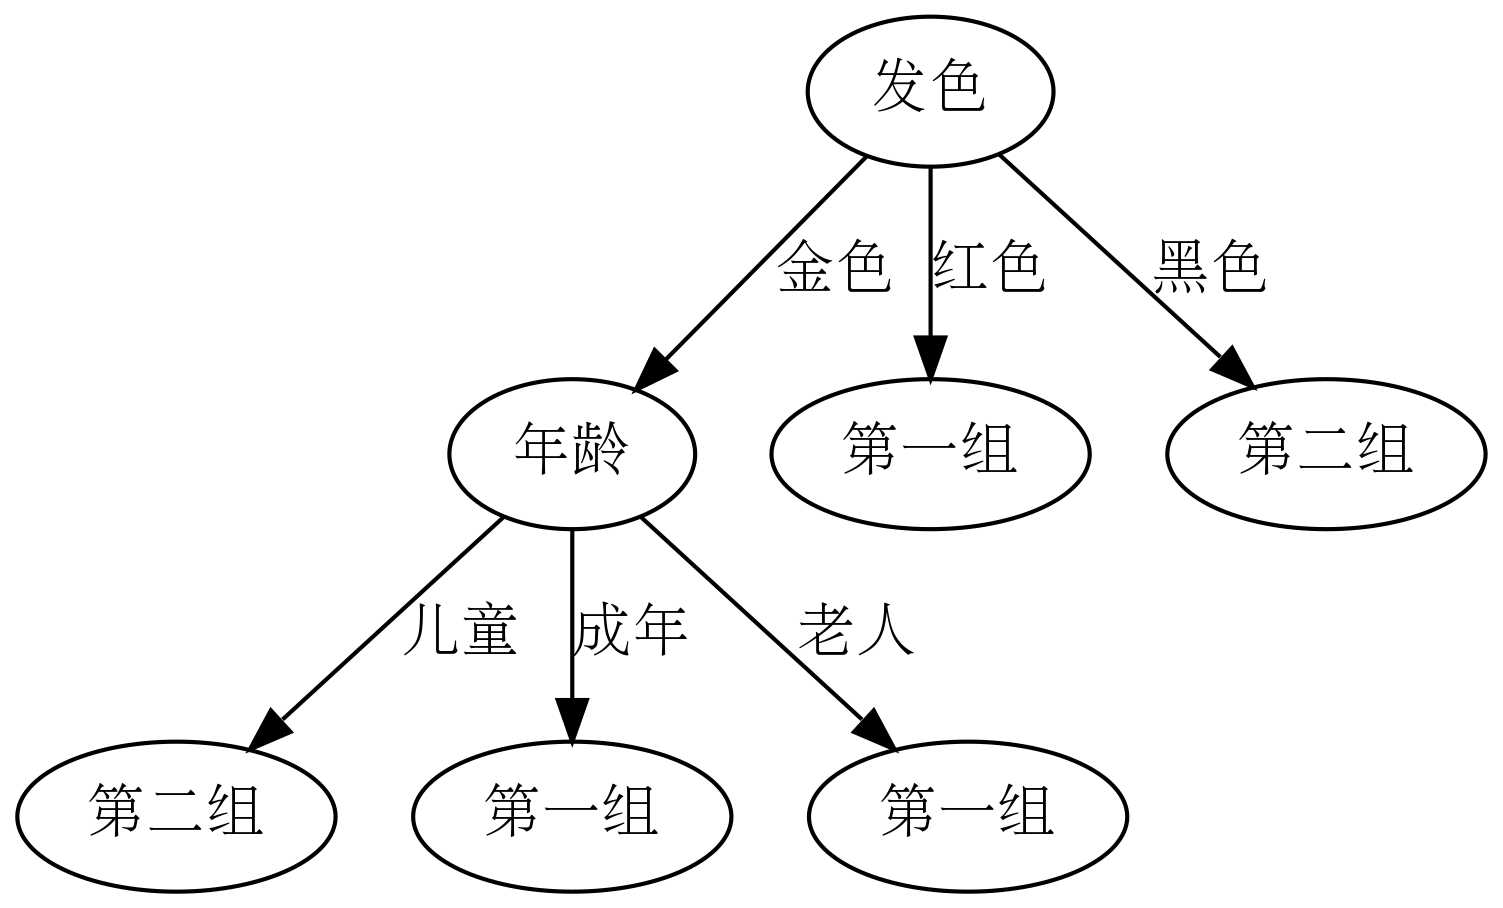
\includegraphics[width=0.6\textwidth]{tree.png}
  \end{center}
    
  \item 用所建分类器说明给定样例(矮,金色,成年)是属于第几组。
  
  第一组。
\end{enumerate}

\section{朴素贝叶斯}

对于上表中的数据:

\begin{enumerate}
  \item 用朴素贝叶斯建立二分类器,写出建立过程(不用考虑平滑)。
  
  \begin{align*}
    P(\text{高}|\text{第一组}) &= 0.5\\
    P(\text{矮}|\text{第一组}) &= 0.5\\
    P(\text{金色}|\text{第一组}) &= 0.75\\
    P(\text{红色}|\text{第一组}) &= 0.25\\
    P(\text{黑色}|\text{第一组}) &= 0\\
    P(\text{儿童}|\text{第一组}) &= 0\\
    P(\text{成年}|\text{第一组}) &= 0.25\\
    P(\text{老人}|\text{第一组}) &= 0.75\\
    P(\text{高}|\text{第二组}) &= 0.6\\
    P(\text{矮}|\text{第二组}) &= 0.4\\
    P(\text{金色}|\text{第二组}) &= 0.2\\
    P(\text{红色}|\text{第二组}) &= 0\\
    P(\text{黑色}|\text{第二组}) &= 0.8\\
    P(\text{儿童}|\text{第二组}) &= 0.4\\
    P(\text{成年}|\text{第二组}) &= 0.2\\
    P(\text{老人}|\text{第二组}) &= 0.4\\
  \end{align*}
  
  \item 用所建分类器对给定样例(矮,金色,成年)分类。
  
  \begin{align*}
    & P(\text{(矮,金色,成年)}|\text{第一组})P(\text{第一组}) \\
    &= P(\text{矮}|\text{第一组})P(\text{金色}|\text{第一组})P(\text{成年}|\text{第一组})P(\text{第一组}) \\
    &= 0.5 * 0.75 * 0.25 * \frac{4}{9} \\
    &= 0.042 \\
    \\
    & P(\text{(矮,金色,成年)}|\text{第二组})P(\text{第二组}) \\
    &= P(\text{矮}|\text{第二组})P(\text{金色}|\text{第二组})P(\text{成年}|\text{第二组})P(\text{第二组}) \\
    &= 0.4 * 0.2 * 0.2 * \frac{5}{9} \\
    &= 0.009
  \end{align*}
  
  故是第一组。
\end{enumerate}

\end{document}